\chapter{Thrust characteristics}

Graphs below present empirical data on the thrust produced by Sadulli Piccino and Sadulli Grosso. 
All data collected at normal conditions: standard atmospheric pressure (100 kPa) and normal temperature (25\degree{}C) at MSL.

\begin{ZubaxTableWrapper}{Propeller characteristics}
    \begin{ZubaxWrappedTable}{| X | X | X | X |}
    Parameter           & Sadulli Piccino   & Sadulli Grosso & Unit \\
    Propeller diameter  & 15                & 17             & inch \\
    Propeller pitch     & 5.5               & 6.2            & inch \\
\end{ZubaxWrappedTable}
\end{ZubaxTableWrapper}

In the realm of constant pitch propeller drives, there is a tendency for thrust efficiency reduction 
with the increase of propeller RPM. This means that although maximum thrust is limited by propeller material 
and motor and controller power limitations and may reach relatively high values,  
it may be beneficial not to use the drive at its maximum thrust levels and stay at relatively low RPM 
where the efficiency is higher. The specific efficiency level proposed for optimum operation is 10 gf/W. 
Aircraft designer should keep that in mind and select the propulsion system accordingly.

\newpage
\section{Sadulli Piccino thrust figures}

\begin{figure}[!hbt]
    \centerline{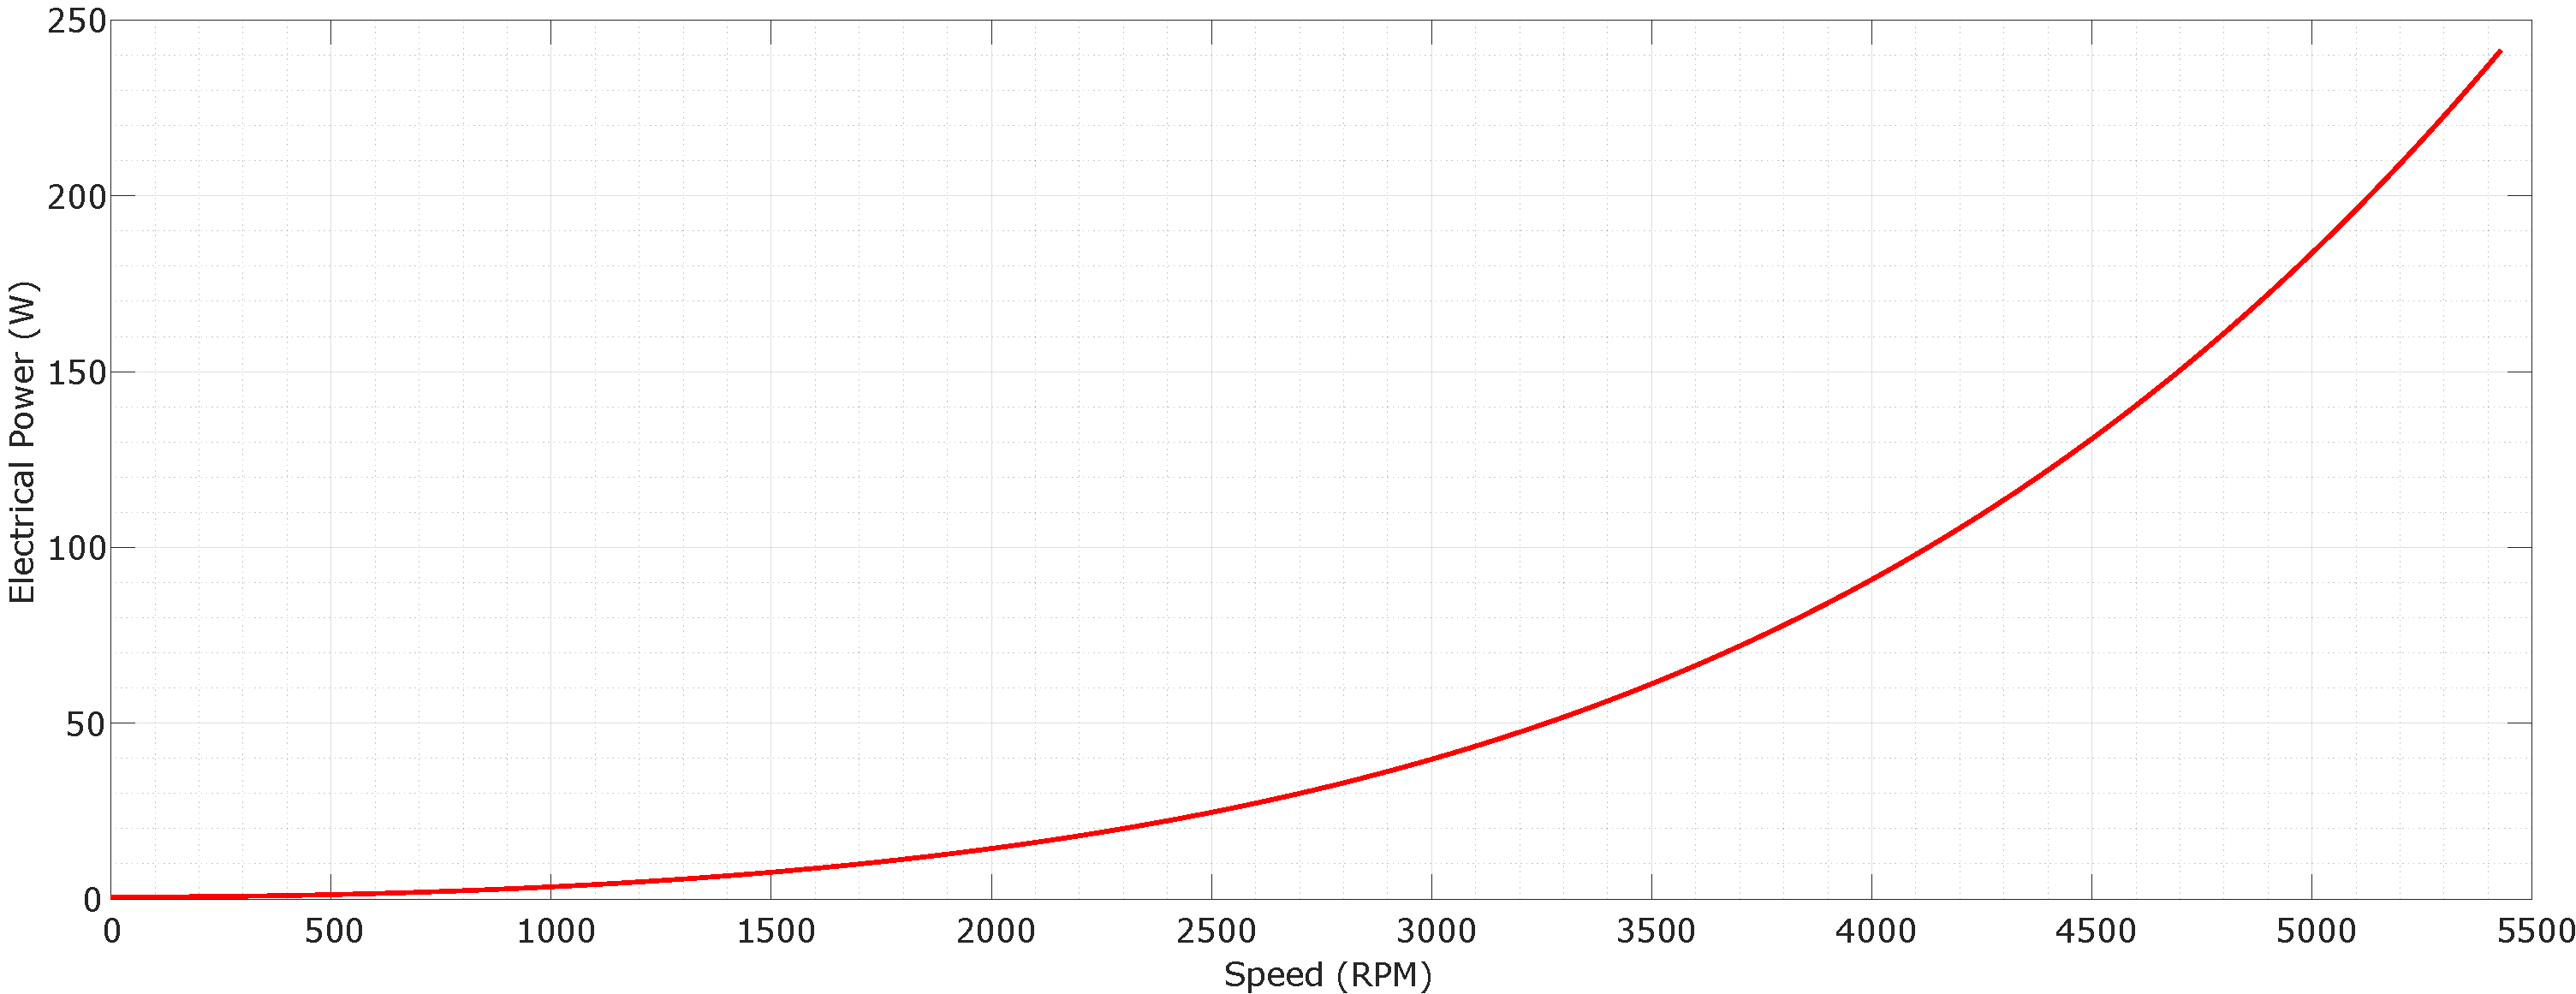
\includegraphics[width=1\textwidth]{figures/thrust_graphs/piccino_power-rpm.pdf}}
    \caption{Sadulli Piccino electrical power vs. RPM}
\end{figure}

\begin{figure}[!hbt]
    \centerline{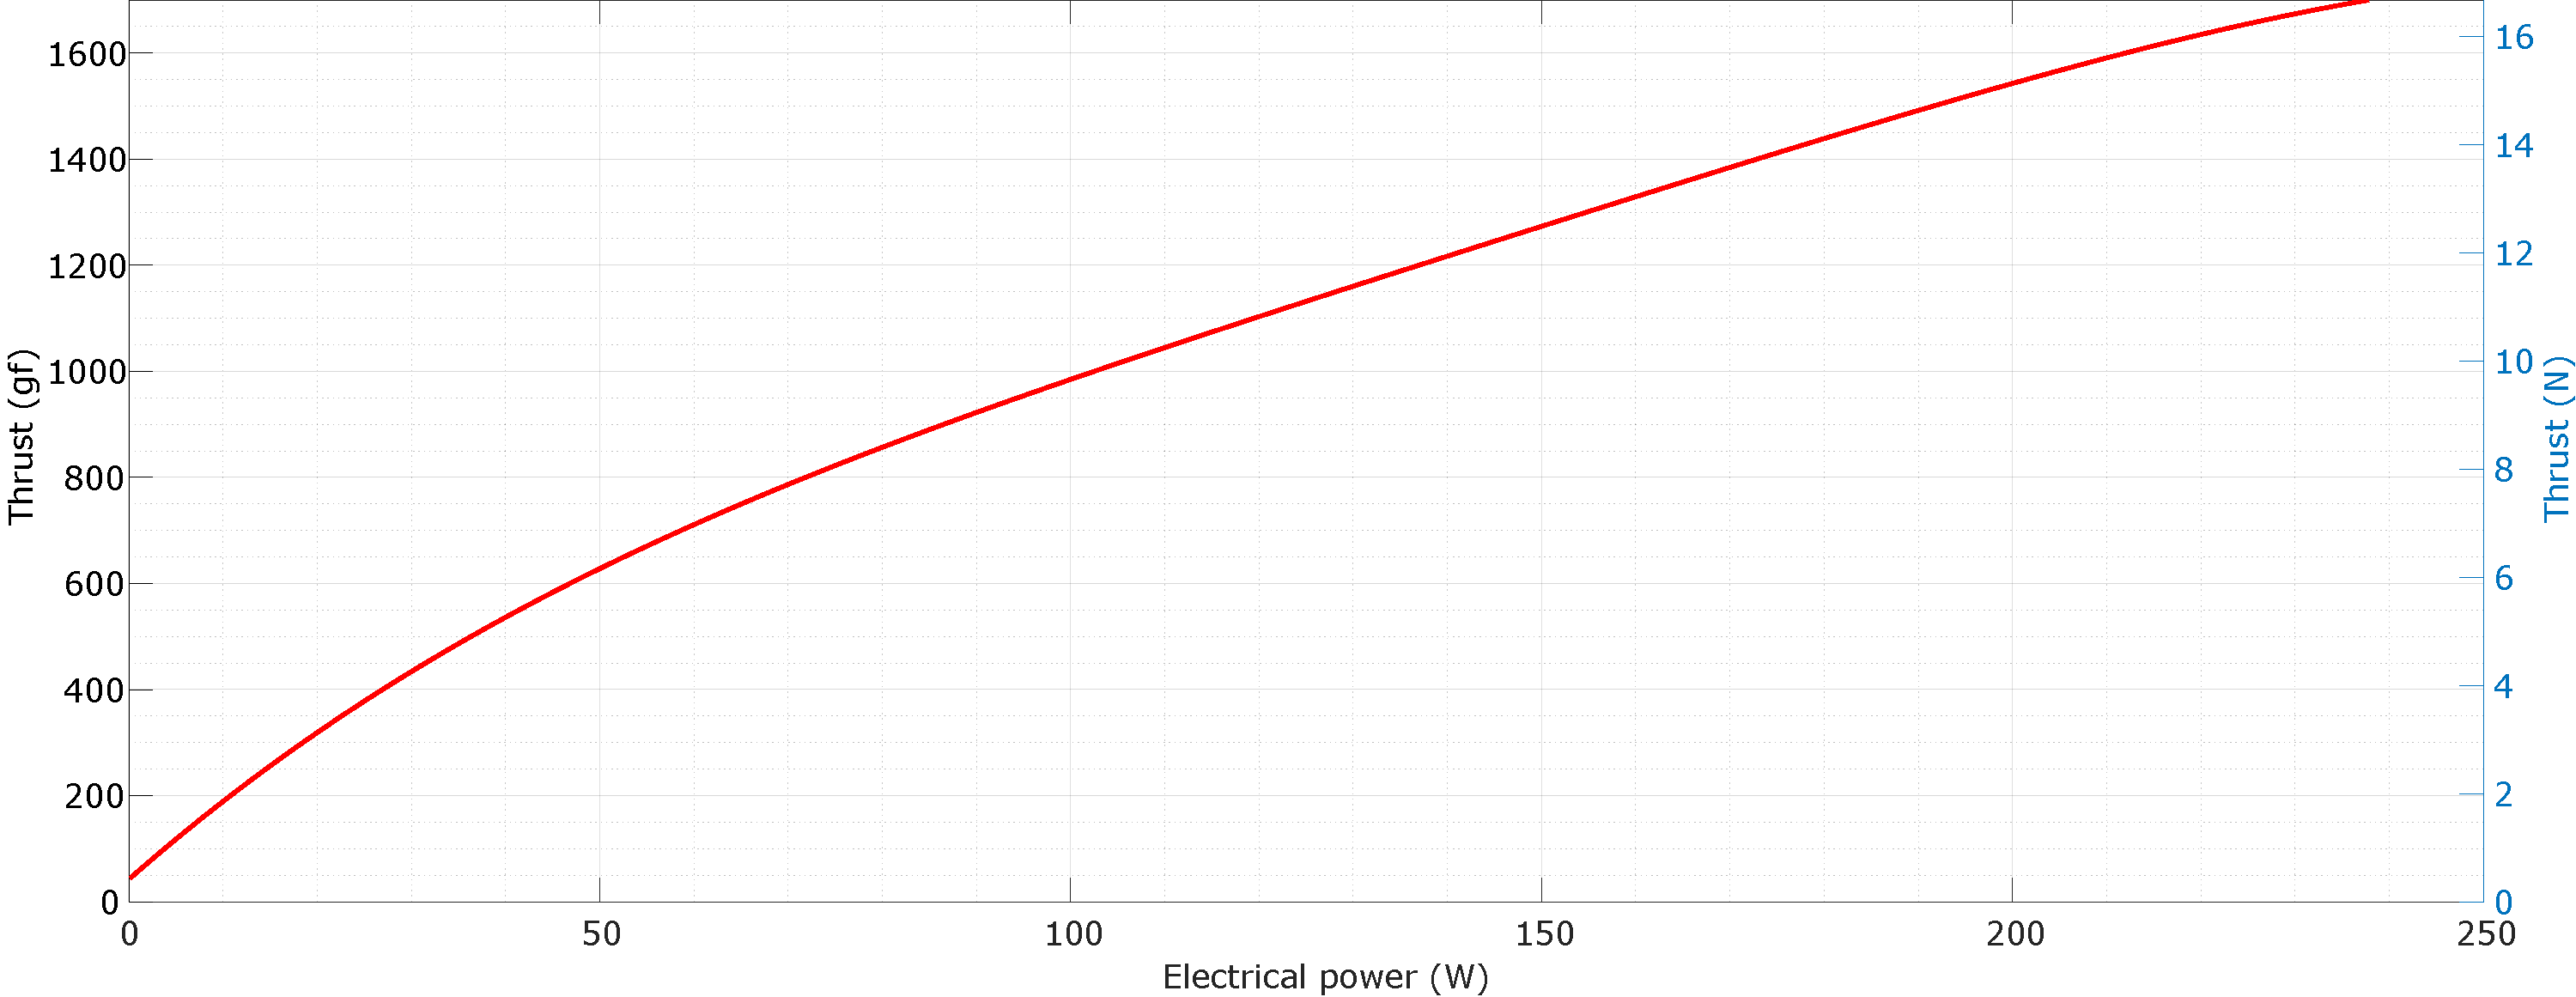
\includegraphics[width=1\textwidth]{figures/thrust_graphs/piccino_thrust-power.pdf}}
    \caption{Sadulli Piccino thrust  vs. electrical power}
\end{figure}

\begin{figure}[!hbt]
    \centerline{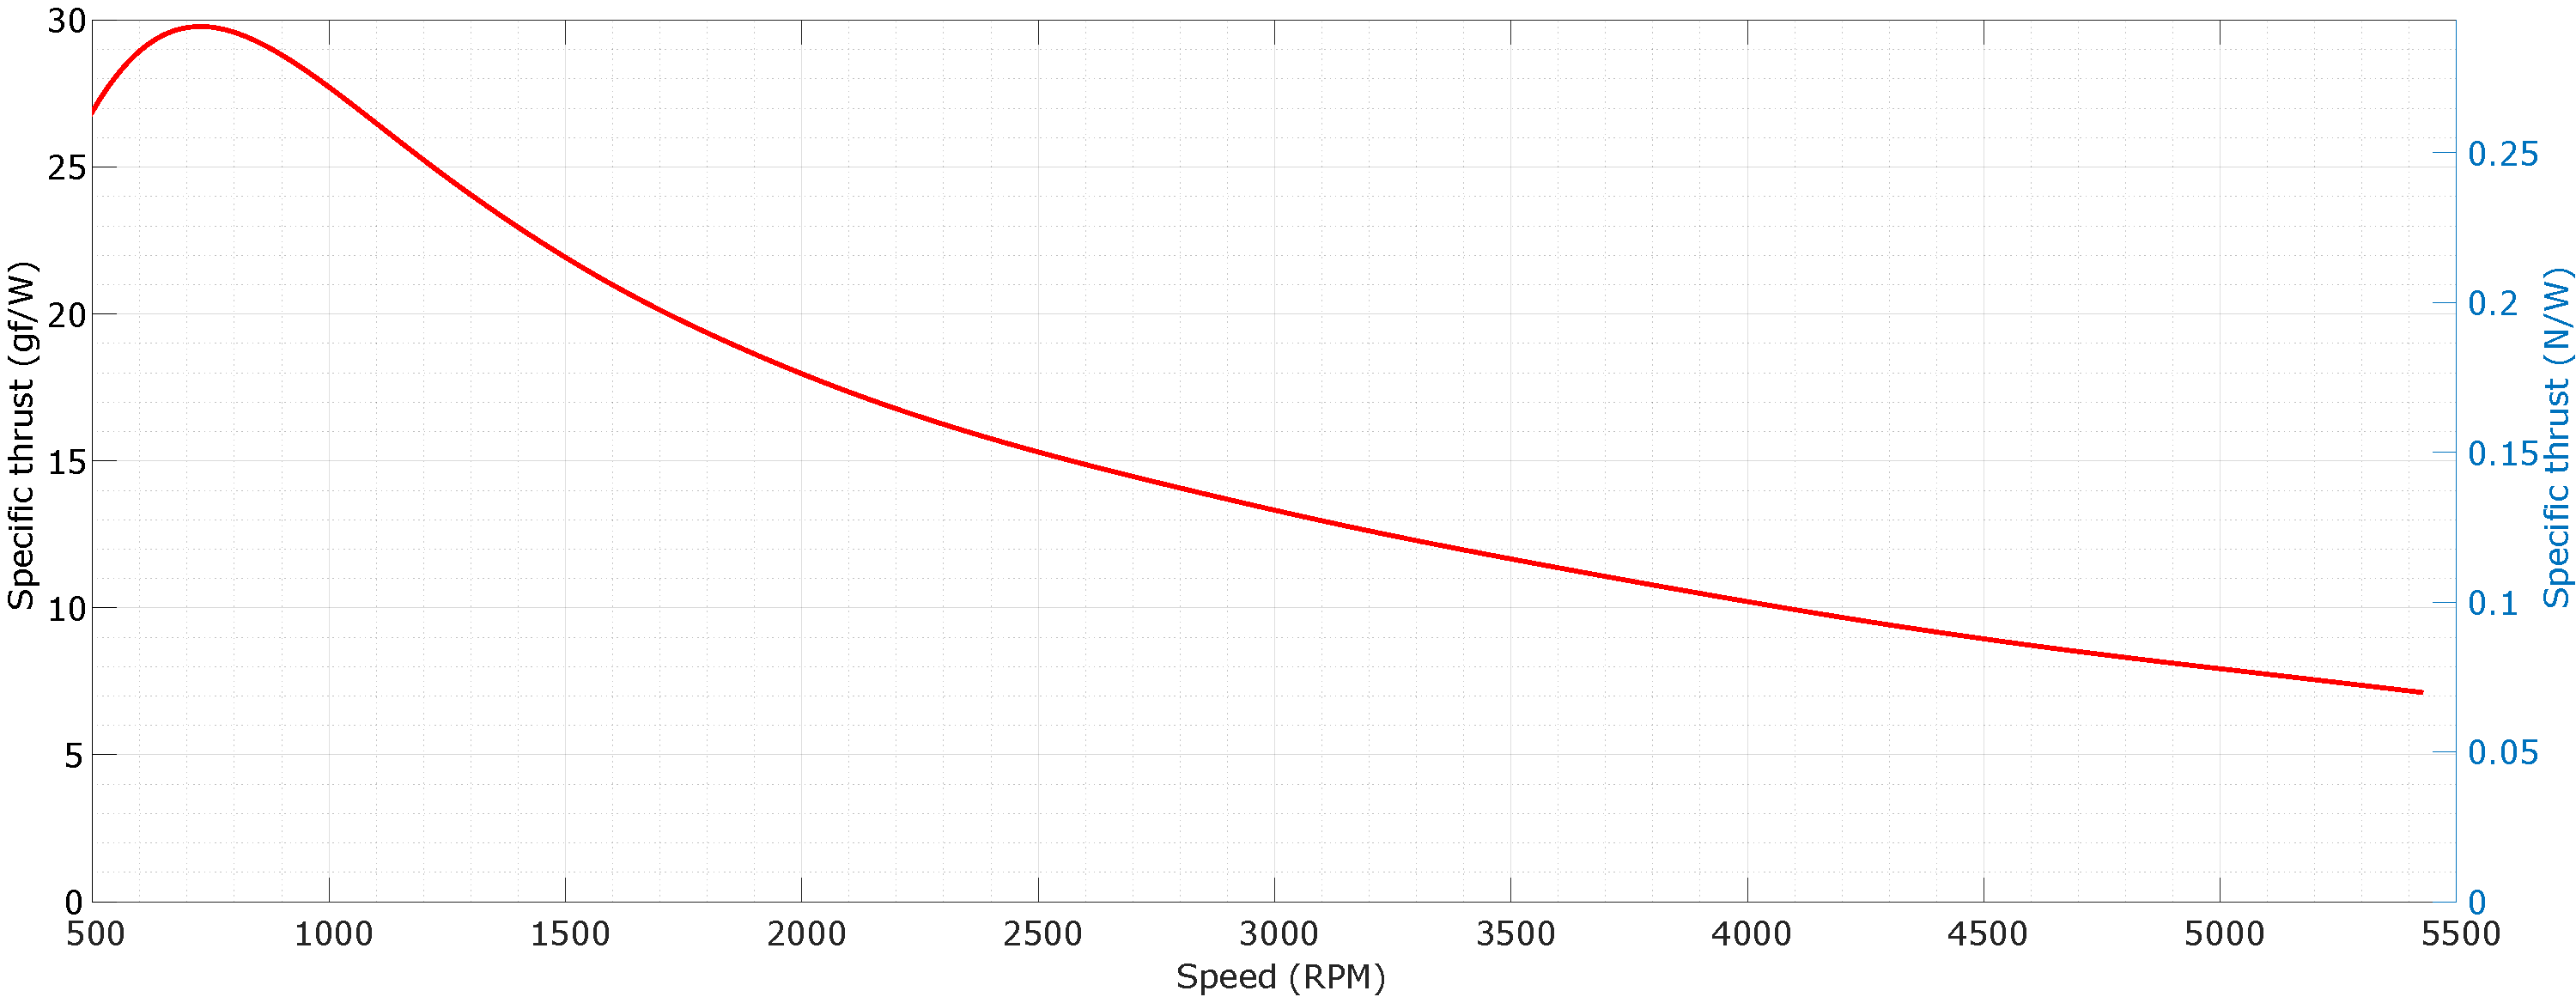
\includegraphics[width=1\textwidth]{figures/thrust_graphs/piccino_specific_thrust-rpm.pdf}}
    \caption{Sadulli Piccino specific thrust vs. RPM}
\end{figure}

\newpage

\section{Sadulli Grosso thrust figures}

\begin{figure}[!hbt]
    \centerline{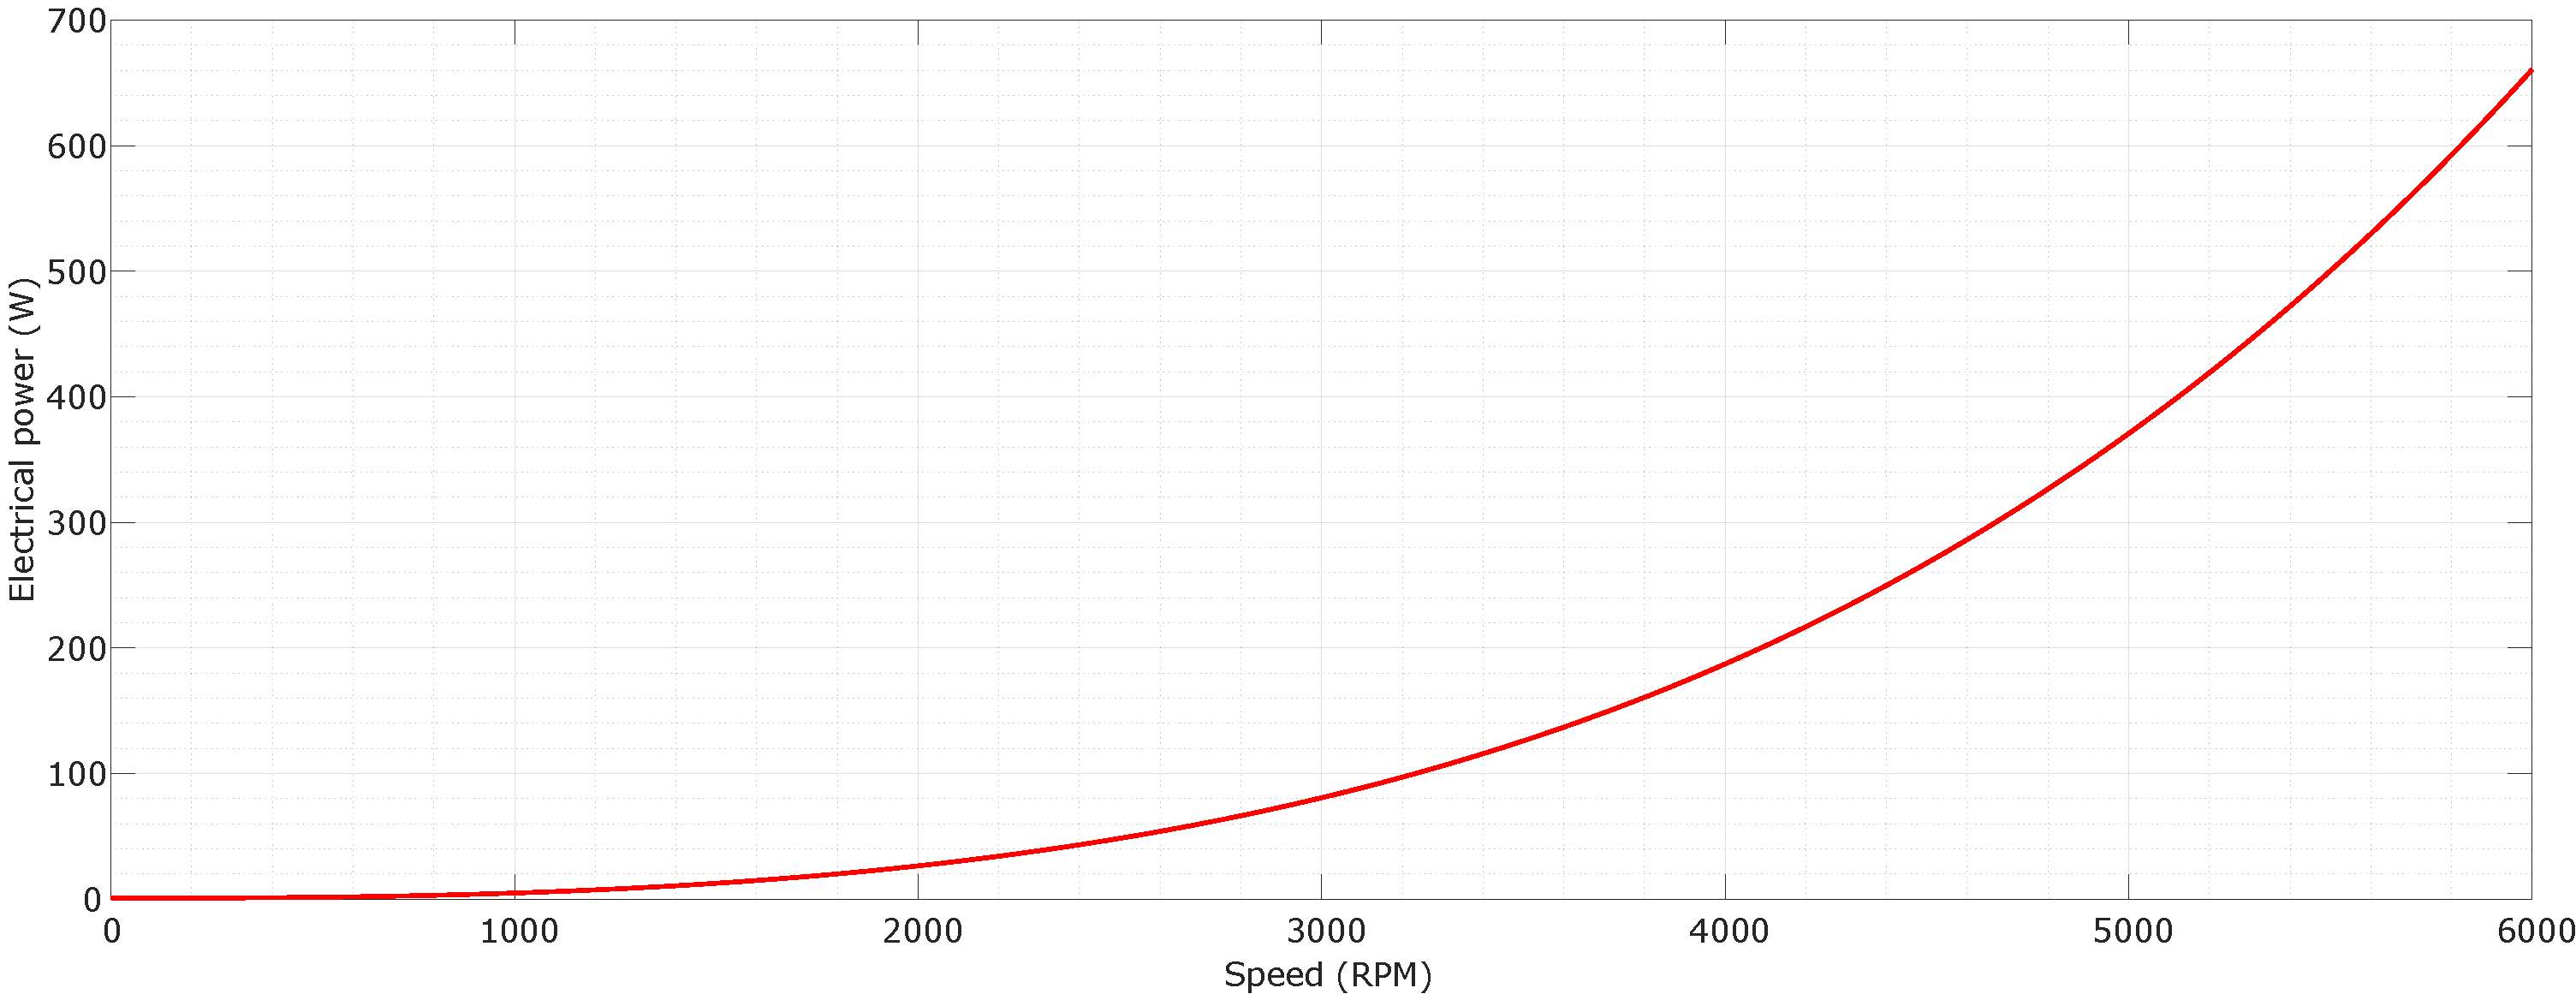
\includegraphics[width=1\textwidth]{figures/thrust_graphs/grosso_power-rpm.pdf}}
    \caption{Sadulli Grosso electrical power vs. RPM}
\end{figure}

\begin{figure}[!hbt]
    \centerline{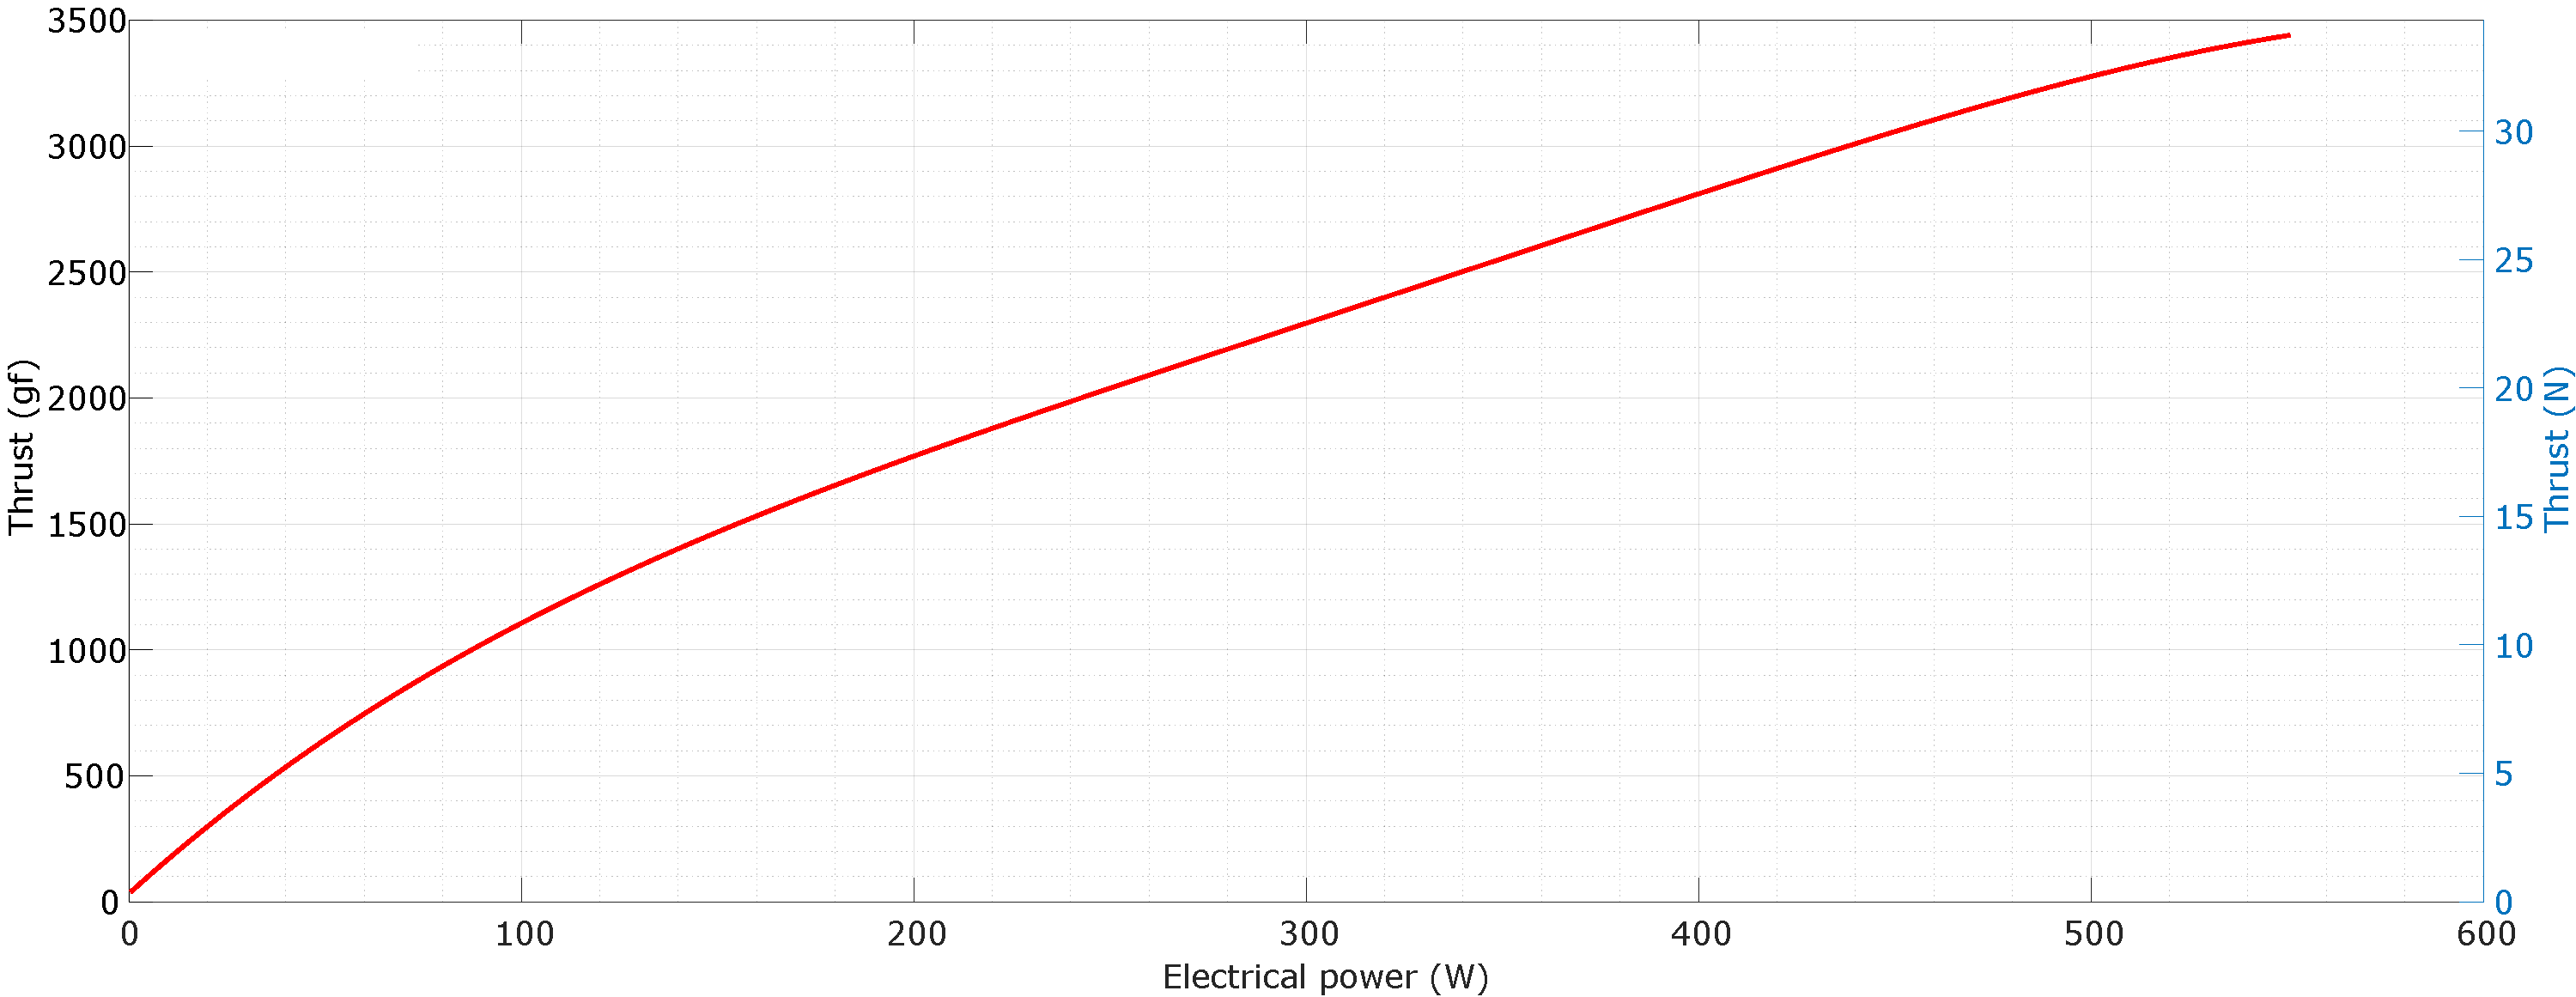
\includegraphics[width=1\textwidth]{figures/thrust_graphs/grosso_thrust-power.pdf}}
    \caption{Sadulli Grosso thrust  vs. electrical power}
\end{figure}

\begin{figure}[!hbt]
    \centerline{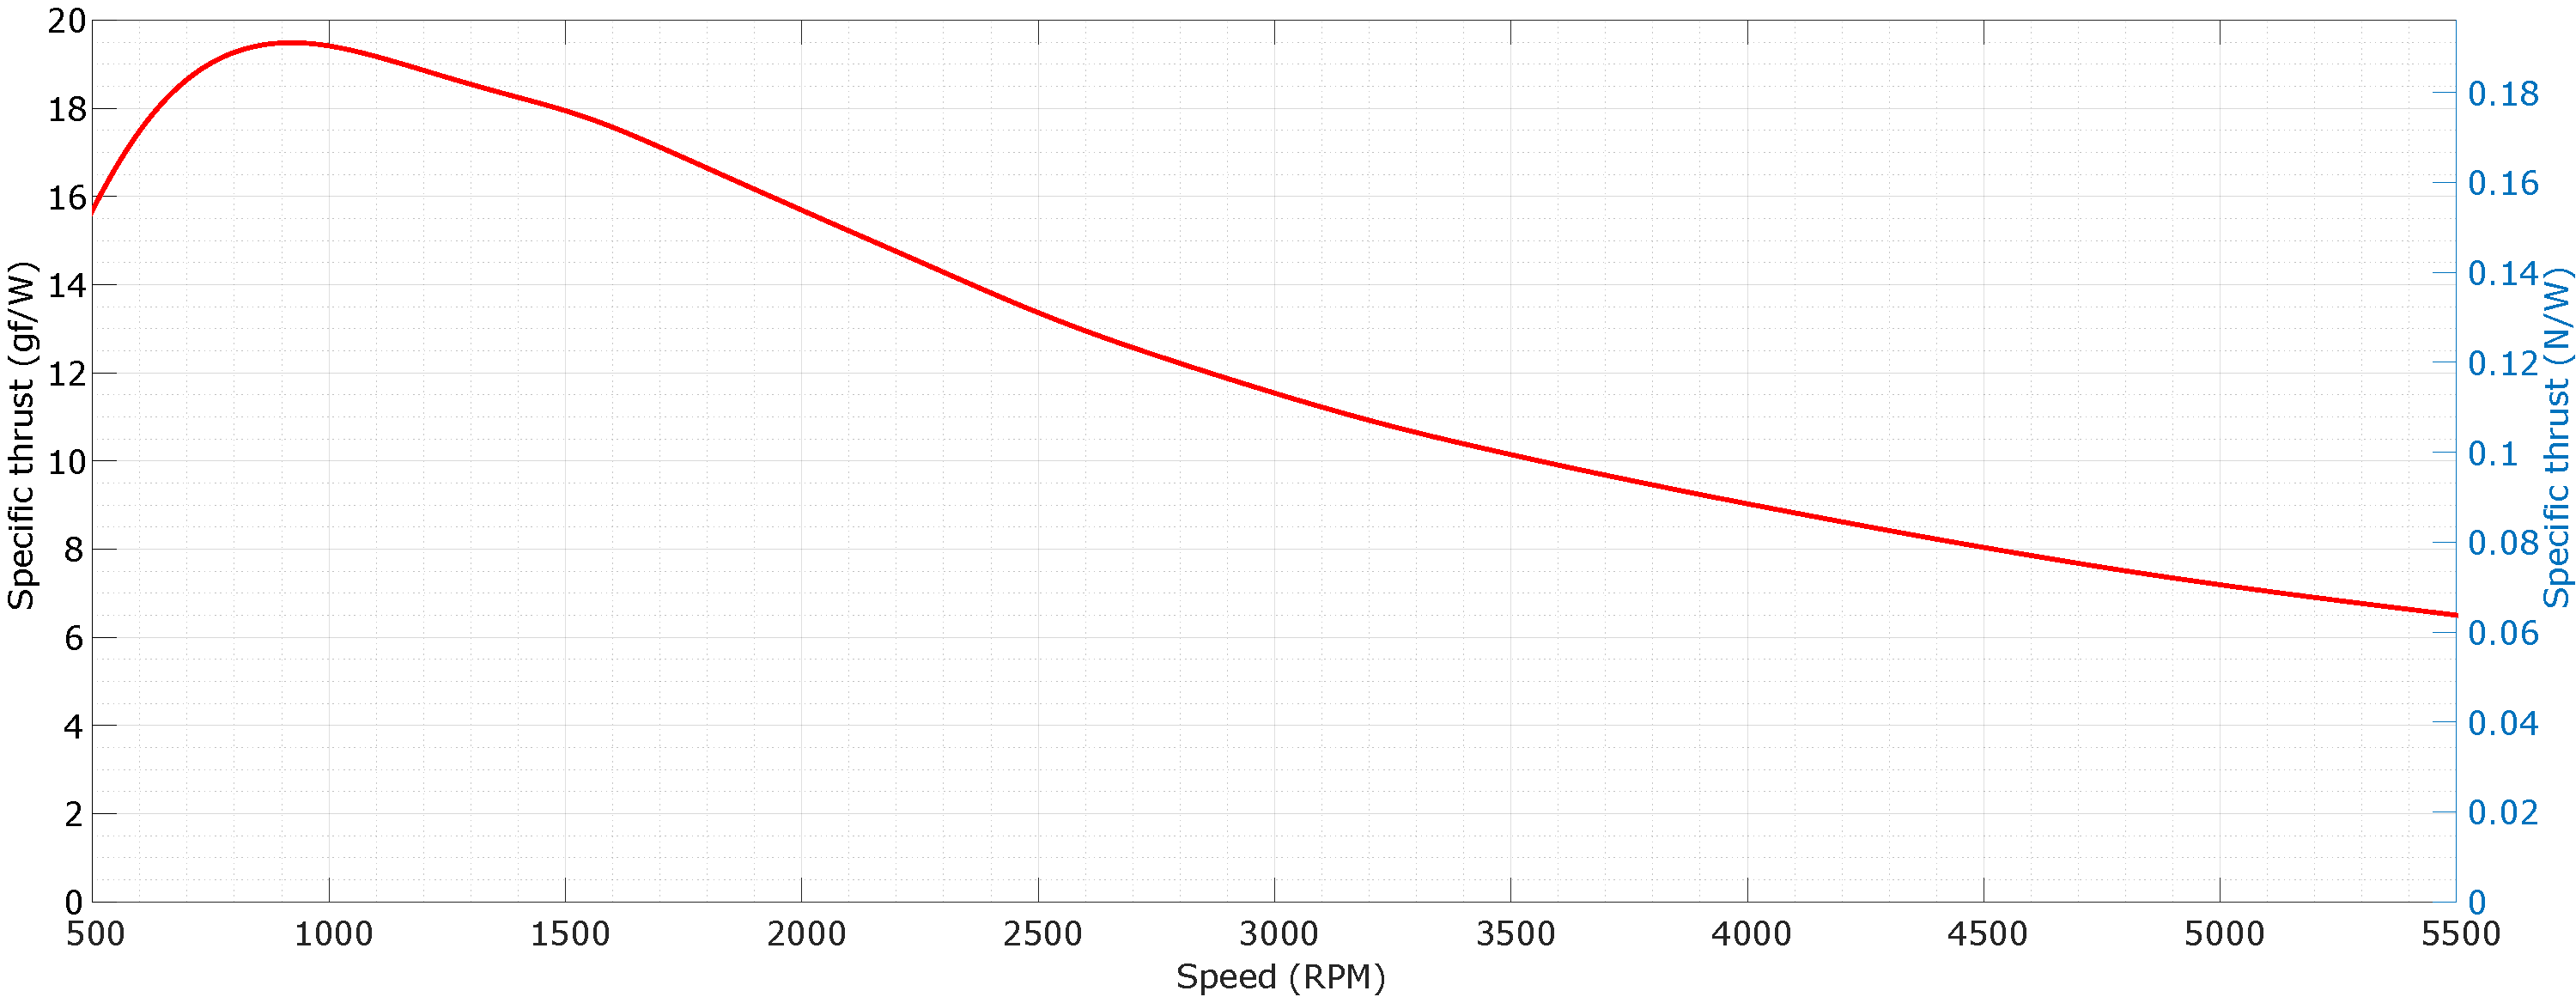
\includegraphics[width=1\textwidth]{figures/thrust_graphs/grosso_specific_thrust-rpm.pdf}}
    \caption{Sadulli Grosso specific thrust vs. RPM}
\end{figure}

\newpage

\subsection{Motor selection considerations}{\label{sec:motor_selection}}

One non-obvious matter that differs FOC-enabled motor controllers (like Sadulli) from conventional controllers with 
trapezoidal or six step commutation is so called voltage utilization factor.
Every BLDC motor has a characteristic that defines its theoretical maximum rotational speed. 
It is called  motor speed constant K\textsubscript{v}. 
It is measured in revolutions per minute (RPM) per volt or radians per volt second [rad/(V*s)].
Physical meaning of this constant is the number of revolutions per minute (rpm) that a motor turns when 1V (one volt) 
is applied with no load attached to that motor. 

FOC-enabled motor controllers have additional voltage utilization factor that decreases the maximum RPM 
for a given motor and supply voltage. For Sadulli this factor is:

\[F\textsubscript{util} = \frac{0.91}{\sqrt{3}}\]
\[RPM\textsubscript{max} = K\textsubscript{v}\ V\textsubscript{supply}\ F\textsubscript{util}\]

RPM\textsubscript{max} of a FOC enabled motor controller will always be lower than RPM\textsubscript{max} 
of a conventional controller with trapezoidal or six step commutation. This should be taken into account 
when designing a propulsion system. 

\newpage

\subsection {Sadulli Piccino/Gross supply voltage considerations}

Although all variants of Zubax Sadulli are designed for operation in the wide supply voltage range it may be beneficial to use the highest admissible supply voltage for Sadulli Piccino/Grosso, i.e. 8S battery in the case of typical $\text{LiCoO}_\text{2}$ battery. There are two reasons for that:

\begin{enumerate}
\item Power losses in the drive are proportional to the square of the phase current. Meanwhile output power is linearly proportional to the phase current. This means that it is energetically favourable to reduce phase current while keeping output power constant. This can be achieved by increasing the supply voltage. 

\item As stated above in section~\ref{sec:motor_selection}, Sadulli utilizes the supply voltage incompletely, which means that it may be impractical to use Sadulli Piccino/Grosso with low supply voltages.
\end{enumerate}

\begin{figure}[!hbt]
    \centerline{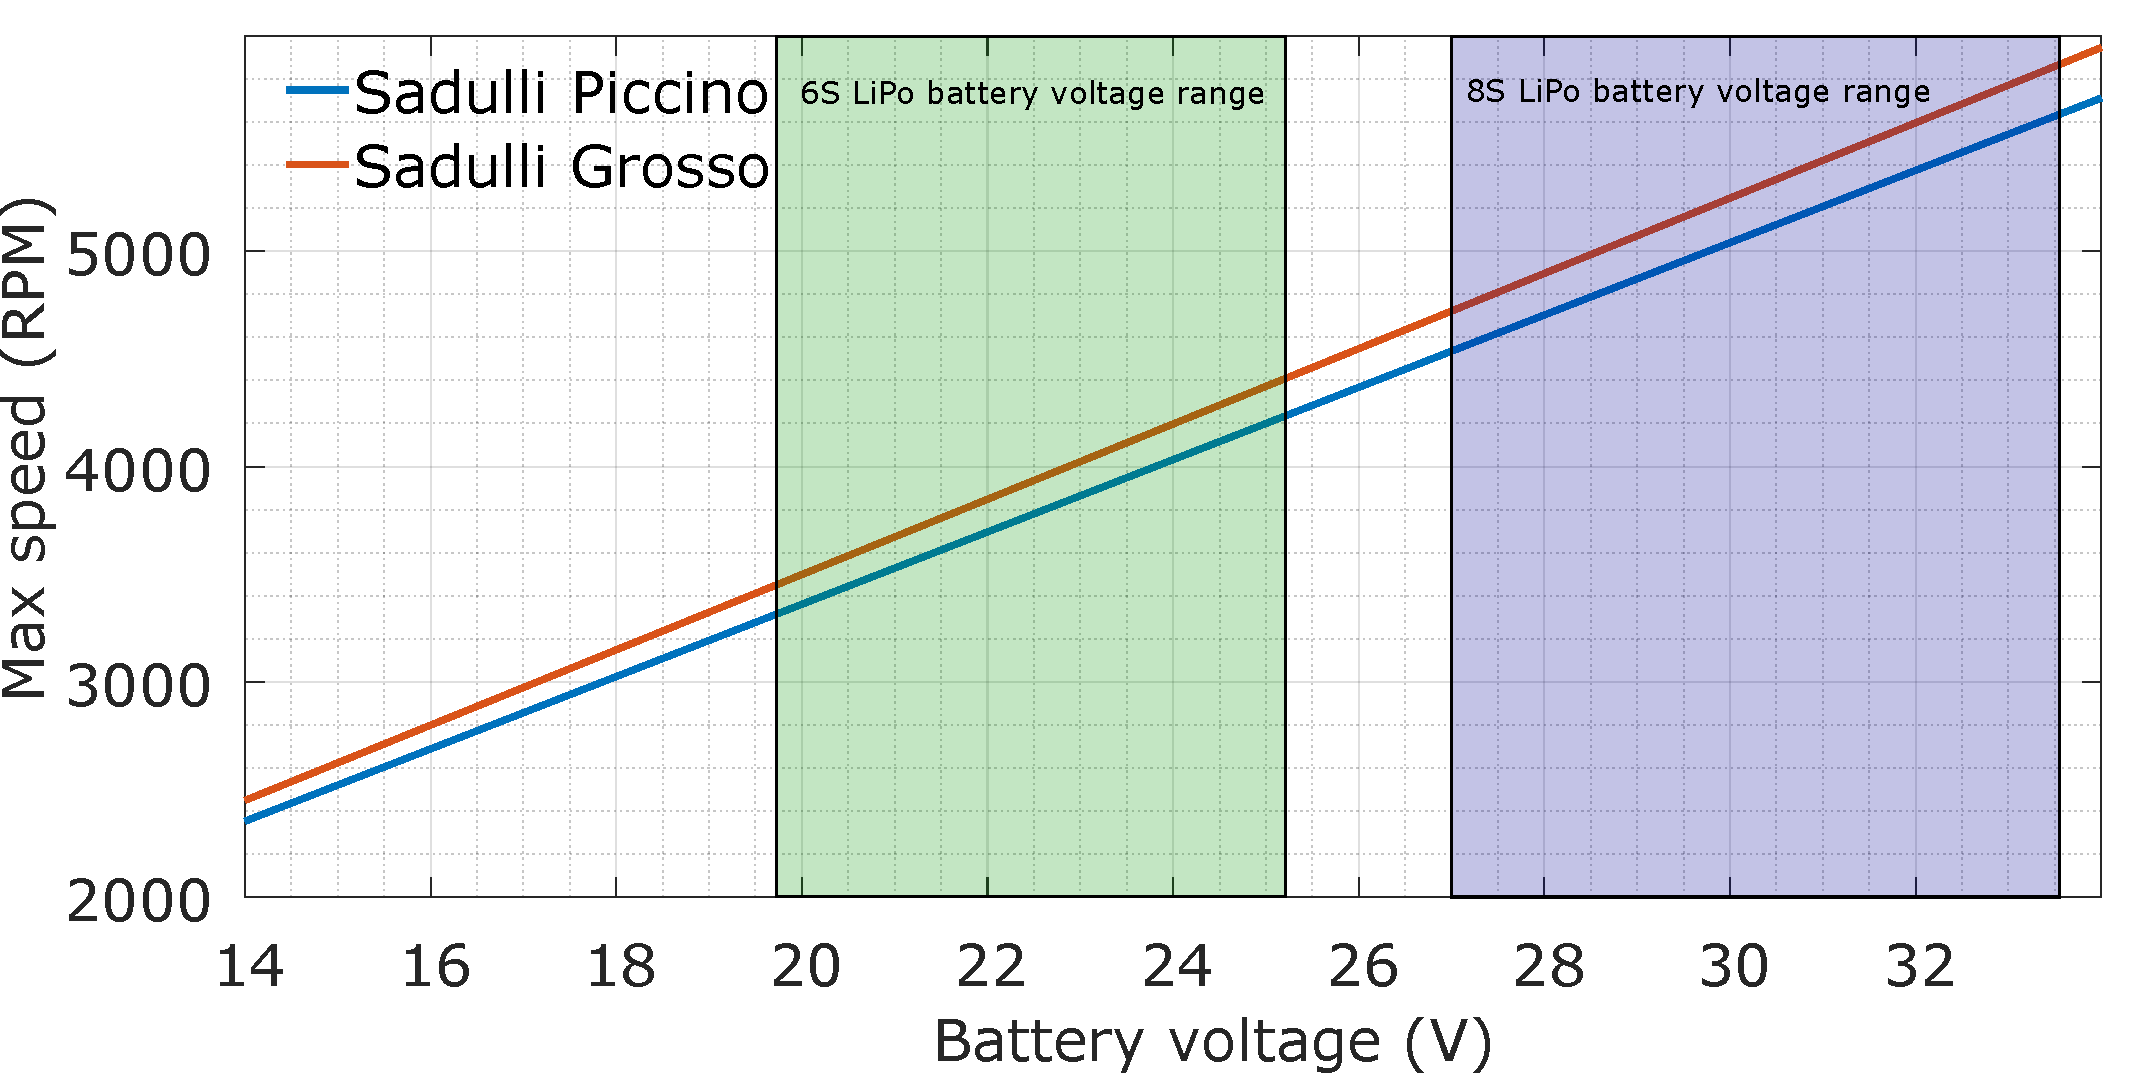
\includegraphics[width=1\textwidth]{figures/thrust_graphs/maxrpm_vs_voltage.pdf}}
    \caption{Sadulli Piccino/Grosso maximum RPM vs. supply voltage}
\end{figure}

\begin{figure}[!hbt]
    \centerline{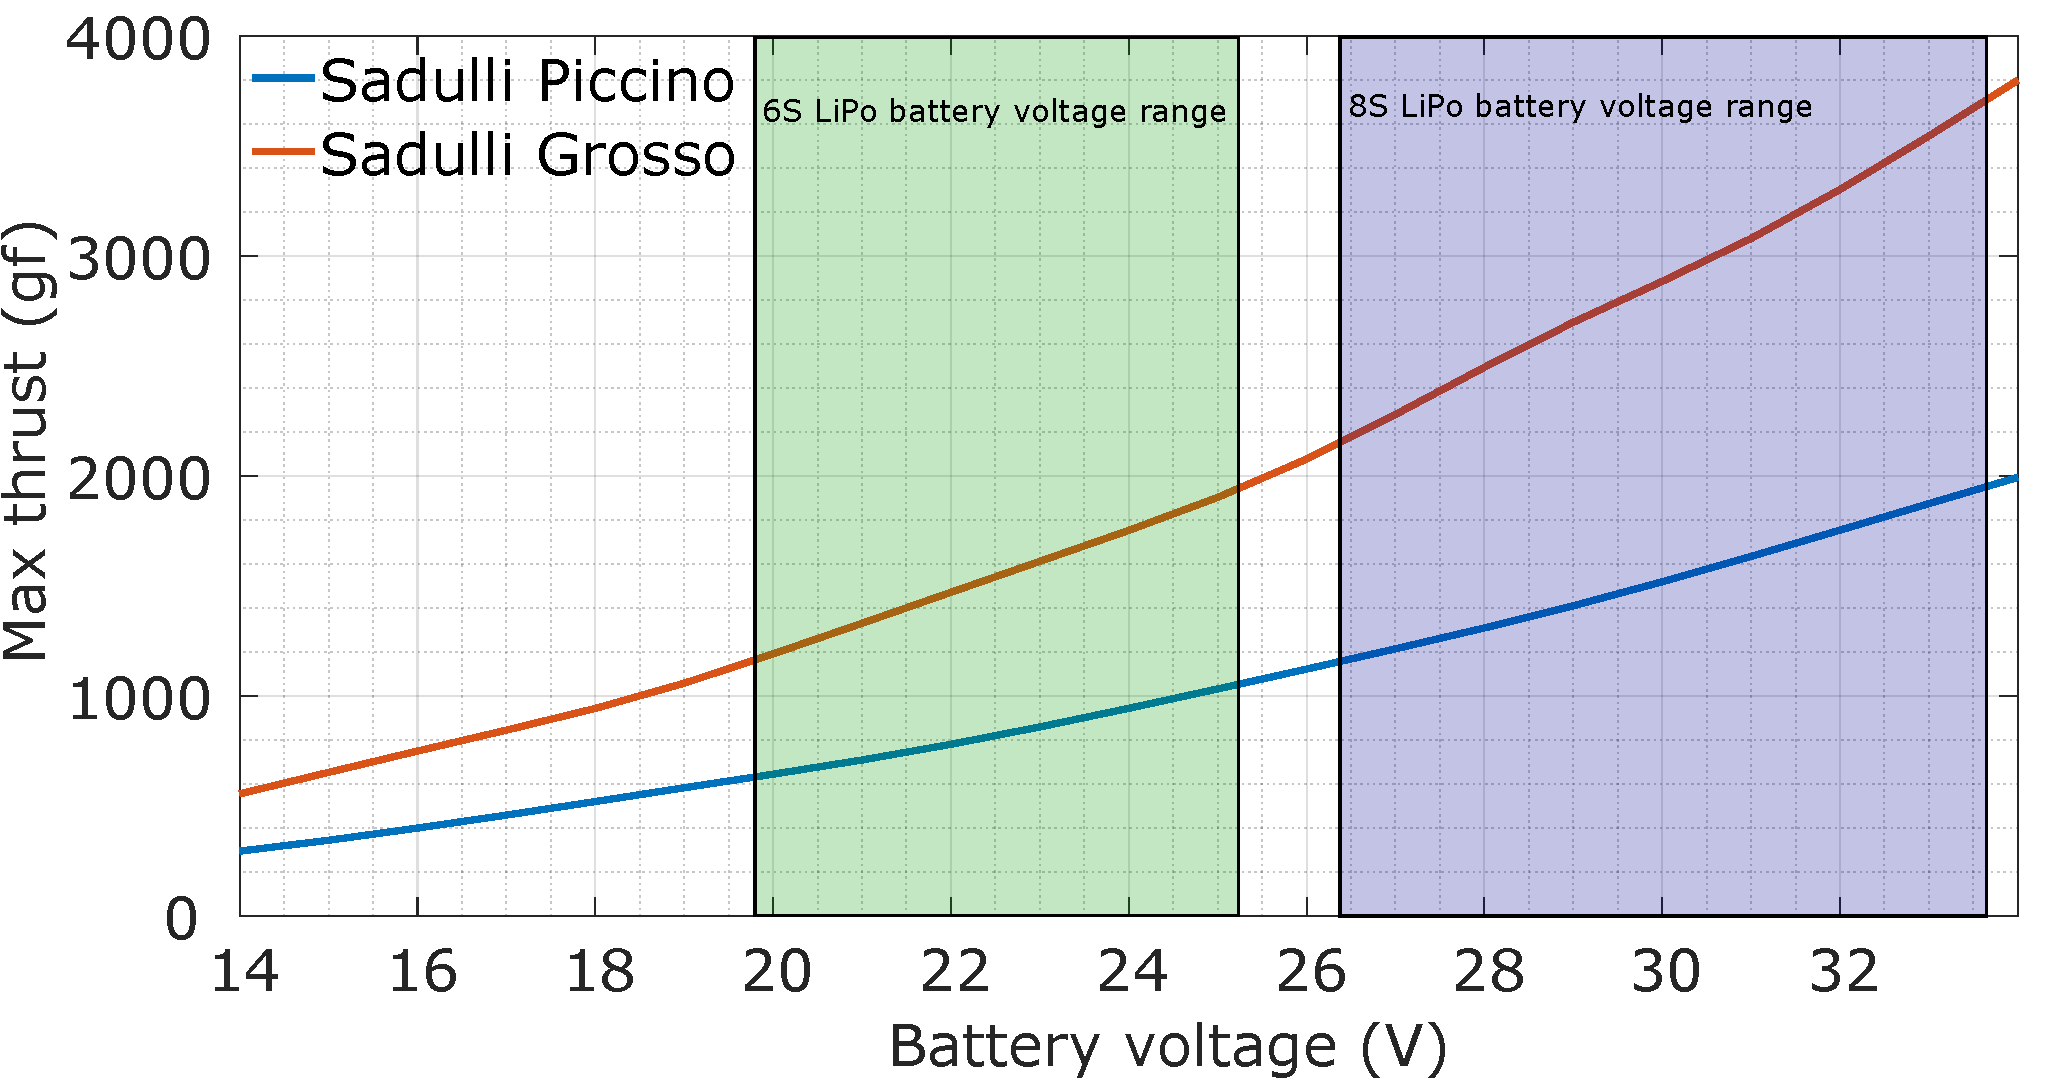
\includegraphics[width=1\textwidth]{figures/thrust_graphs/maxthrust_vs_voltage.pdf}}
    \caption{Sadulli Piccino/Grosso maximum thrust vs. supply voltage}
\end{figure}
